% Intended LaTeX compiler: pdflatex
\documentclass[koma,a4paper,utopia,12pt,listings-color,microtype,paralist,colorlinks,urlcolor=red]{org-article}
       \usepackage{tikz}
       \usetikzlibrary{arrows,decorations.pathmorphing}
       \usetikzlibrary{backgrounds,positioning,fit,petri}
               \usepackage{tikz}
\author{Eason}
\date{\today}
\title{Set up the TikZ in Emacs Org}
\hypersetup{
 pdfauthor={Eason},
 pdftitle={Set up the TikZ in Emacs Org},
 pdfkeywords={},
 pdfsubject={An introduction to setup the TikZ environment in Emacs Org File. So that in Org file, you can generate either vector graph of \texttt{pdf}  format or raster graph of \texttt{png} format. Furthermore, you can export the vector graph when latex is called and otherwise raster graph.},
 pdfcreator={Emacs 26.3 (Org mode 9.2.6)},
 pdflang={English}}
\begin{document}


 \begingroup
\begin{center}
 \vspace{\baselineskip}
 \textbf{\Huge Walk Through the Petri-Net In TiKZ Tutorial} \par
 \vspace{2\baselineskip}  \newline
 \textbf{\large Eason Zhang with www.makesteamclear.com \par}
 \vspace{\baselineskip} \newline
  \today \par
 \vspace{\baselineskip}
  \vfill
 \setlength{\unitlength}{3pt}
 \includegraphics[width=0.5\textwidth]{/Users/chaolongzhang/Dropbox/mstemc_hugo/static/img/tikz/petrinetfinal.pdf}
 \vfill \vspace{\baselineskip}
 \href{WWW.MAKESTEAMCLEAR.COM}{\Large WWW.MAKESTEAMCLEAR.COM} \par\newline
  makesteamclear is a free project, run by Eason Zhang, to make videos about STEAM in a more approachable way. If you find the contents in this article or the site or the youtube channel helpful, please consider \href{www.makesteamclear.com}{support me}, thanks \par
 \end{center}
 \endgroup

 \newpage \textbf{copyright page} \newpage \tableofcontents \newpage

\hspace{0pt}\\


An introduction to setup the TikZ environment in Emacs Org File. So that in Org file, you can generate either vector graph of \texttt{pdf}  format or raster graph of \texttt{png} format. Furthermore, you can export the vector graph when latex is called and otherwise raster graph.


\section{config the header args}
\label{sec:orga783c72}


You can embed TiKz (One of \(\LaTeX\) graphic package) code into a Org file. With
org-babel, you can generate ,insert and export the figure generated from Tikz
package. At first, you need set up the environment. \href{https://orgmode.org/worg/org-contrib/babel/languages/ob-doc-LaTeX.html}{This Post} serves as a good
introduction for beginners. Following it you may have a minimum working example
like below:

\begin{verbatim}
#+name: tutorial
#+header: :file "~/Dropbox/mstemc_hugo/static/img/tikz/tutorial.png"
#+header: :results raw :exports none :fit yes :border 0cm
#+header: :imagemagick t :iminoptions -density 400
#+header: :imoutoptions -geometry 400 -flatten
#+header: :headers '("\\usepackage{tikz} \\usetikzlibrary{positioning,
           shapes.symbols, calc}")
#+begin_src latex
  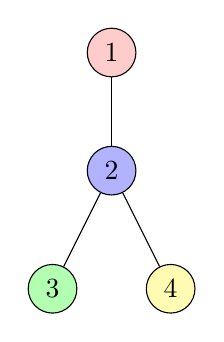
\begin{tikzpicture}
    \node [circle, draw, fill=red!20] at (0,0) {1}
    child { node [circle, draw, fill=blue!30] {2}
      child { node [circle, draw, fill=green!30] {3} }
      child { node [circle, draw, fill=yellow!30] {4} }};
  \end{tikzpicture}
#+end_src
#+RESULTS: tutorial
[[file:../../img/tikz/tutorial.png]]
\end{verbatim}

The example begins with several lines containing \texttt{\#+header} which is sort of
clutter. we can put them in a file and include it at the beginning of the Org
file.
\section{generate results with different formats}
\label{sec:org39c9b75}


By changing the extension of \texttt{:file} (which is \texttt{pdf} for
\texttt{"../../img/tikz/tutorial.pdf"} ), we can generate results with different formats.
Now, I need \texttt{pdf} and \texttt{png} . You can see the result by just press \texttt{C-c C-c} in the
body of the tikz code.
\section{export the results according to the backend}
\label{sec:org58238bf}


You can set \texttt{:exports} to control how the results will be exported. Now I set it
as \texttt{none} which means the result will not be exported to latex or other format. I
want to set more options of the exports. So I use:

\begin{verbatim}
#+ATTR_HTML:  :width 800 :align center
#+ATTR_LATEX: :width 0.8\textwidth :align center
{{{if-latex(tutorial.pdf,tutorial.png)}}}
\end{verbatim}

\texttt{if-latex} is a Org MACRO whose definition is :
\begin{verbatim}
#+MACRO: if-latex (eval (if
(org-export-derived-backend-p org-export-current-backend 'latex)
 (concat "[[file:../../img/tikz/"  $1 "]]")
 (concat "[[file:../../img/tikz/"  $2 "]]") ))
\end{verbatim}

The \texttt{if-latex} MACRO let you export different formats by the backend. If the
backend is \texttt{latex} then, \texttt{pdf} format figure will be exported. Otherwise, \texttt{png} format
figure. Eventually, in the final \texttt{pdf} document, you figure can be zoomed in or
out without losing any resolution.

\section{the final workflow}
\label{sec:org0400fae}


The minimum working example at the start of this post is simplifed as below.

\begin{verbatim}
#+header: :file  "../../img/tikz/tutorial.pdf"
#+begin_src latex
  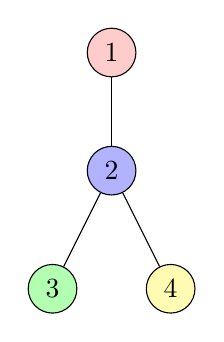
\begin{tikzpicture}
    \node [circle, draw, fill=red!20] at (0,0) {1}
    child { node [circle, draw, fill=blue!30] {2}
      child { node [circle, draw, fill=green!30] {3} }
      child { node [circle, draw, fill=yellow!30] {4} }};
  \end{tikzpicture}
#+end_src

#+RESULTS:
[[file:../../img/tikz/tutorial.png]]

The following is the generated figure.
#+ATTR_HTML:  :width 800 :align center
#+ATTR_LATEX: :width 0.8\textwidth :align center
{{{if-latex(tutorial.pdf,tutorial.png)}}}
\end{verbatim}

Many settings are grouped into a setup file which is included at the top of this
post:
\begin{verbatim}
#+SETUPFILE: ~/.spacemacs.d/org-templates/math-en.org
\end{verbatim}

Now, If you set the extension of the target file in the first line either \texttt{pdf} or
\texttt{png} , a corresponding \texttt{pdf} or \texttt{png} figure will be generated. If execute \texttt{M-x
org-toggle-inline-images}  , you can preview the result. If export the org-file
as latex file then the \texttt{pdf} file, the image of \texttt{pdf} format will be inserted. If
export to other format, \texttt{png} image will be used.
\end{document}
